\documentclass[border=6pt,tikz]{standalone}
\usepackage{tikz}
\usepackage{amsmath,amssymb}
\usetikzlibrary{arrows.meta,positioning,fit,backgrounds,calc,shapes.geometric,decorations.pathreplacing,patterns}
\definecolor{ink}{HTML}{1B2430}
\definecolor{muted}{HTML}{6B7785}
\definecolor{accent}{HTML}{2F6FB5}
\definecolor{accent2}{HTML}{C1611F}
\definecolor{good}{HTML}{2E7D5B}
\definecolor{soft}{HTML}{EDF2F7}
\definecolor{soft2}{HTML}{FBEDE2}
\definecolor{soft3}{HTML}{E6F0E9}
\tikzset{
  box/.style={draw=ink,line width=.7pt,rounded corners=2pt,fill=soft,inner sep=4pt,align=center,font=\sffamily\small},
  boxa/.style={box,fill=soft2},
  boxb/.style={box,fill=soft3},
  plain/.style={align=center,font=\sffamily\small,text=ink},
  tiny/.style={align=center,font=\sffamily\scriptsize,text=muted},
  ar/.style={-{Stealth[length=2.4mm]},draw=ink,line width=.7pt},
  arm/.style={-{Stealth[length=2.4mm]},draw=muted,line width=.6pt,dashed},
  nd/.style={circle,draw=ink,line width=.7pt,fill=white,minimum size=7mm,inner sep=0pt,font=\sffamily\scriptsize},
  ndf/.style={nd,fill=soft},
  ndt/.style={nd,fill=soft2},
}

\begin{document}
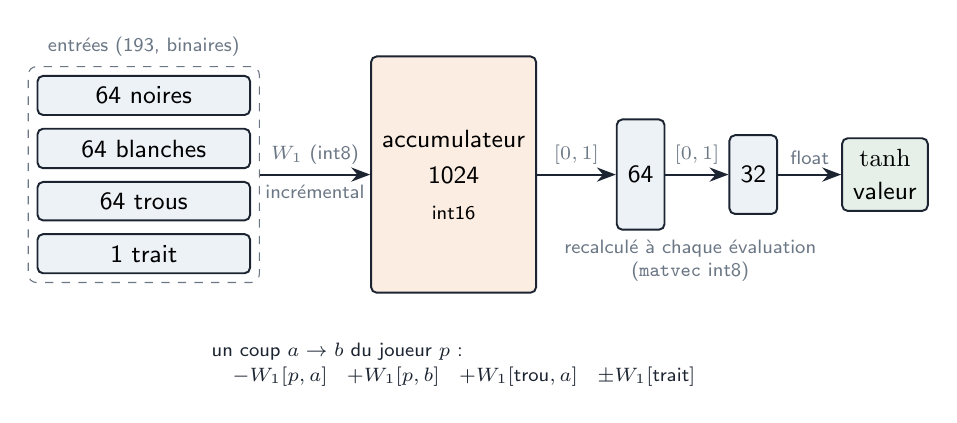
\begin{tikzpicture}[node distance=7mm]
  % inputs
  \node[box,minimum width=27mm] (b) {64 noires};
  \node[box,minimum width=27mm,below=1.5mm of b] (w) {64 blanches};
  \node[box,minimum width=27mm,below=1.5mm of w] (e) {64 trous};
  \node[box,minimum width=27mm,below=1.5mm of e] (t) {1 trait};
  \node[fit=(b)(t),draw=muted,dashed,rounded corners=3pt,inner sep=3pt,label={[tiny]above:entrées (193, binaires)}] (in) {};
  % accumulator
  \node[boxa,right=14mm of in,minimum height=30mm,minimum width=20mm] (acc) {accumulateur\\[2pt]1024\\[2pt]\scriptsize int16};
  \draw[ar] (in) -- node[tiny,above]{$W_1$ (int8)} node[tiny,below]{incrémental} (acc);
  % clamp + layers
  \node[box,right=10mm of acc,minimum height=14mm] (h2) {64};
  \node[box,right=8mm of h2,minimum height=10mm] (h3) {32};
  \node[boxb,right=8mm of h3] (v) {$\tanh$\\[1pt]valeur};
  \draw[ar] (acc) -- node[tiny,above]{$[0,1]$} (h2);
  \draw[ar] (h2) -- node[tiny,above]{$[0,1]$} (h3);
  \draw[ar] (h3) -- node[tiny,above]{float} (v);
  \node[tiny,below=2mm of h3,xshift=-8mm] {recalculé à chaque évaluation\\(\texttt{matvec} int8)};
  % update
  \node[tiny,below=5mm of acc,align=left,text=ink] (up) {un coup $a\to b$ du joueur $p$ :\\[1pt]
    \quad $-W_1[p,a]$ \; $+W_1[p,b]$ \; $+W_1[\text{trou},a]$ \; $\pm W_1[\text{trait}]$};
\end{tikzpicture}
\end{document}
